\documentclass[11pt, a4paper]{article}
\usepackage[margin=1in]{geometry}
\usepackage{amsfonts, amsmath, amssymb}
\usepackage{graphicx}
\parindent 0pt

\title{Orbit Mania}
\author{Adriel Imaran Santoso (C2TB1701)}
\date{\today}

\renewcommand{\thesection}{\Roman{section}}

\begin{document}
\maketitle

\section{Introduction}
"Orbit Mania" is a space-themed arcade game where the player controls a spacecraft, dodging asteroids while managing fuel consumption. This report provides an overview of the game's objectives, background inspiration, theoretical concepts, and code explanation.\\[6pt]
This game was inspired by the concept of the Hohmann transfer, which I encountered last spring break while exploring my curiosity about orbital mechanics. It refers to a space maneuver used to transfer a spacecraft between two orbits of different radii about a central body while conserving fuel.

\section{How to Play}
\subsection{Objective}
The goal is to navigate the spacecraft through an asteroid field while avoiding collisions and managing the fuel bar to prevent depletion. Players can also switch between two circular orbits, where energy packets are scattered to provide slight fuel refills.

\subsection{Controls}
The game makes use of the following keys:
\begin{itemize}
\item \textbf{ESC}: Quit the game
\item \textbf{SPACE}: Switch between orbits
\item \textbf{s}: Activate shield (must be held pressed)
\end{itemize}

\subsection{Objects}
The game features the following elements:
\begin{itemize}
\item \textbf{Planet}
\item \textbf{Player}
\item \textbf{Obstacle}
\item \textbf{Energy packet}
\item \textbf{Shield}
\end{itemize}
Refer to Figure 1 and 2 for in-game snapshots of these objects.

\begin{figure}[h]
\centering
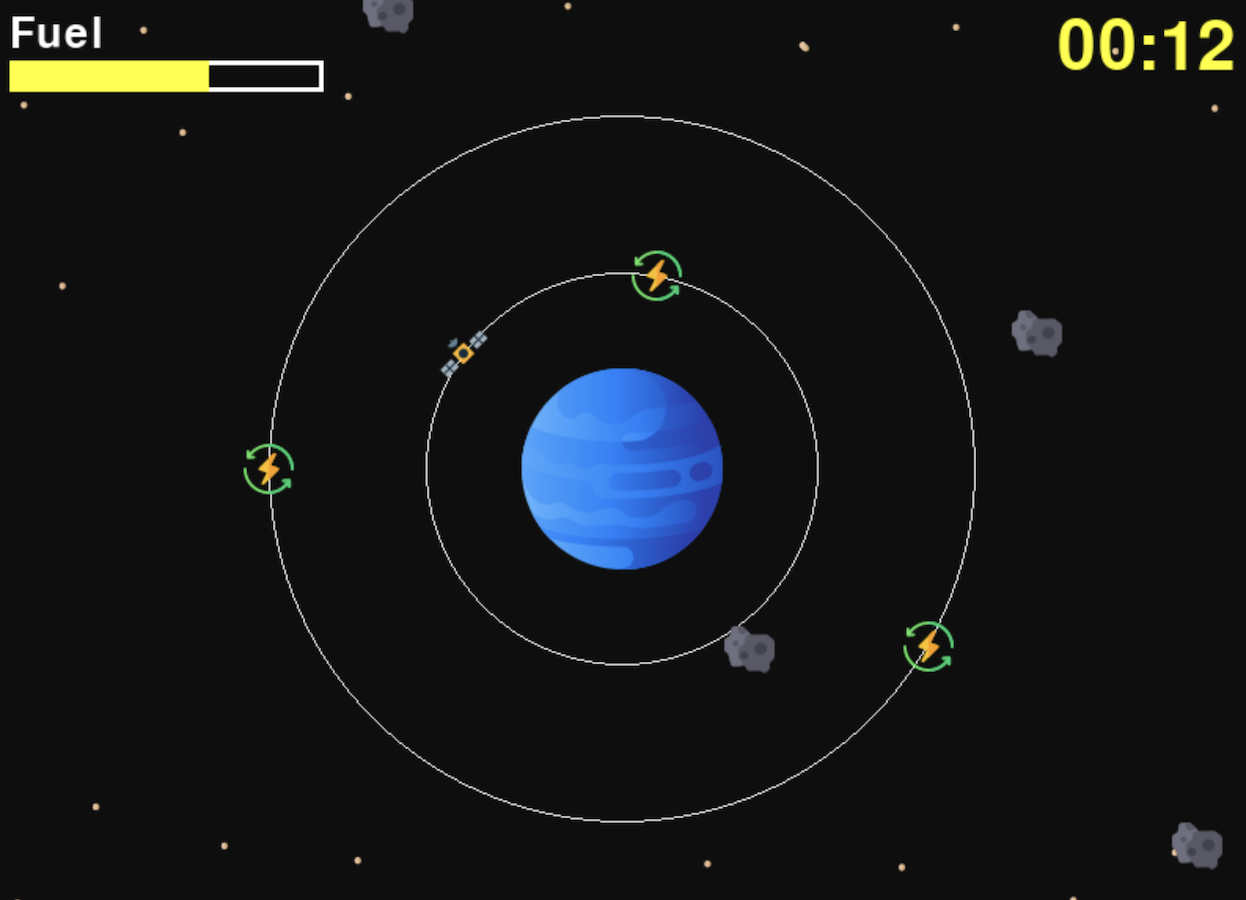
\includegraphics[scale=0.5]{figure1}
\caption{Game objects: planet, player, obstacles, and energy packets}
\end{figure}

\section{Theoretical Background}
\subsection{The Polar Representation of a Circle}
A circle can be represented parametrically using a vector-valued function
$$f(\theta) = \begin{bmatrix}
r\cos\theta \\
r\sin\theta \end{bmatrix}$$
where $r$ is the radius and $\theta$ varies from 0 to $2\pi$ radians for a full cycle.

\subsection{Circular Orbits}
Circular orbits happen when the gravitational force equals the centrifugal force,
$$\dfrac{GMm}{r^2}=\dfrac{mv^2}{r},$$
where $G$ represents the gravitational constant, $M$ is the mass of the central body (such as a planet or star), $m$ is the mass of the orbiting object (e.g., a satellite), $r$ denotes the radius of the orbit, and $v$ signifies the orbital velocity of the object. This results in
$$v=\sqrt{\dfrac{GM}{r}}.$$

\subsection{The Hohmann Transfer}
In astronautics, the Hohmann transfer enables a spacecraft to switch from one circular orbit to another through two consecutive fuel thrusts. The first thrust initiates an elliptical orbit, followed by the second to enter the new circular orbit. Moreover, the ellipse transition orbit completes after $\pi$ radians.

\section{Code Explanation}

\subsection{orbit\_mania.py}
This file contains the game's core functionality, including object classes, player movement, and game mechanics.

\begin{enumerate}
\item The \texttt{World} class is defined with an \texttt{\_\_init\_\_} function that initializes the game environment, including setting the width and height of the screen, loading images and background music, and setting up sounds.
\item The \texttt{Planet} class represents the celestial body around which the player orbits. It includes functions for drawing the orbit path and updating its position.
\item The \texttt{Player} class represents the player-controlled object in the game. It includes functions for movement control, orbit switching, and interaction with other game elements. Methods for activating and deactivating the shield are also included.
\item The \texttt{Shield} class represents the protective barrier around the player. It includes functions for activation, deactivation, and visual representation on the screen.

\vspace{10pt}
\begin{figure}[h]
\centering
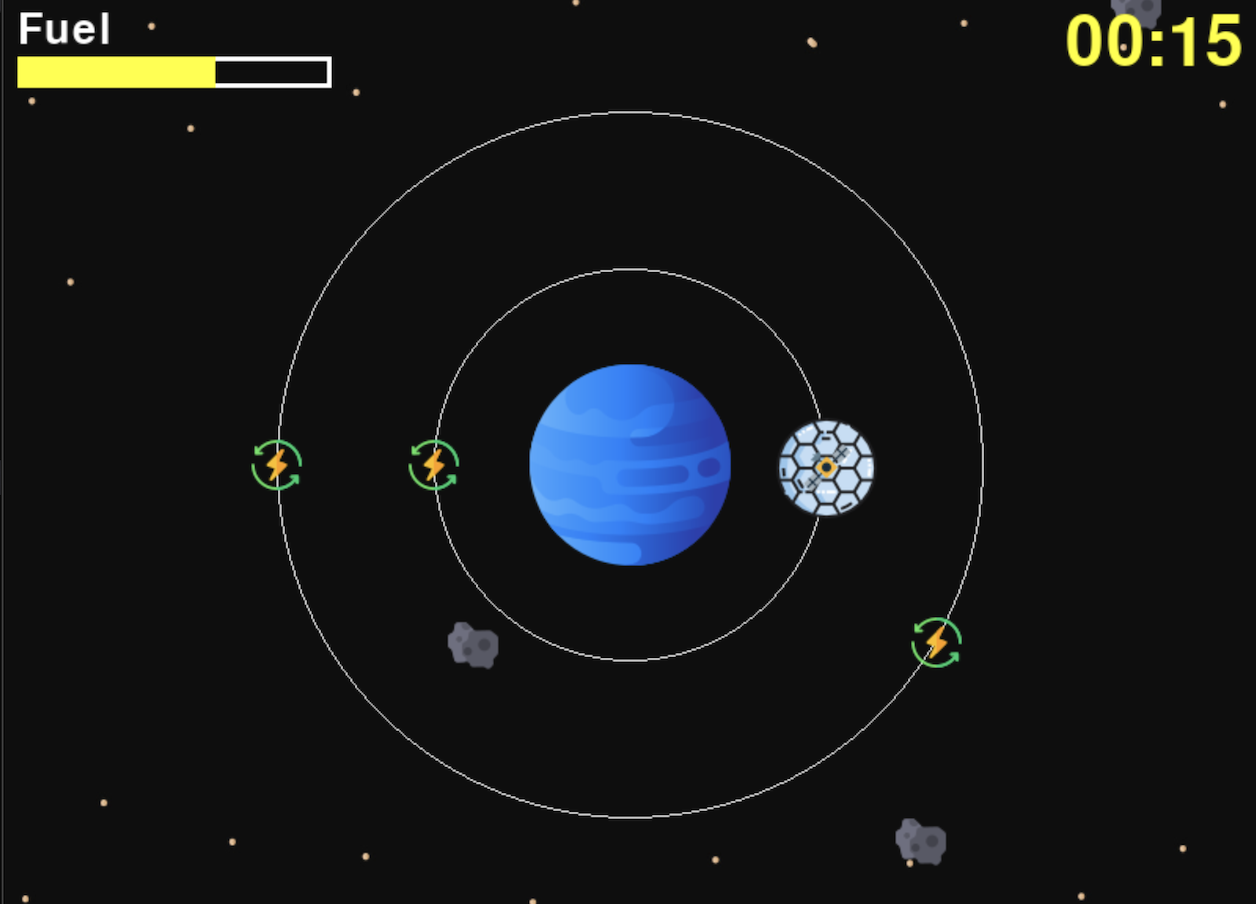
\includegraphics[scale=0.5]{figure2}
\caption{Shield functionality}
\end{figure}

\item The \texttt{FuelBar} class represents the player's fuel level. It includes functions for updating the fuel level based on player actions and collisions with energy packets.
\item The \texttt{EnergyPacket} class represents the collectible items that replenish the player's fuel. It includes functions for spawning at random locations and interacting with the player's fuel bar.
\item Lastly, the \texttt{Obstacle} class is defined, responsible for generating obstacles within the game environment. It includes attributes such as position and speed, along with methods for updating and drawing obstacles on the screen.
\end{enumerate}

\subsection{main.py}
This file initializes the game environment and manages the game loop, event handling, and game over conditions.

\begin{enumerate}
\item The \texttt{AppMain} class is defined with an \texttt{\_\_init\_\_} function that initializes the game environment, including creating instances of the \texttt{World}, \texttt{Planet}, \texttt{FuelBar}, and \texttt{Player} classes, as well as initializing sprite groups for obstacles and energy packets.
\item Inside the \texttt{\_\_init\_\_} function of the \texttt{AppMain} class, various attributes such as the game screen, fonts, images, sounds, and time-related variables are set up.
\item The \texttt{format\_time} function formats the elapsed time into minutes and seconds for display purposes.
\item The \texttt{add\_obstacle} function generates random obstacles at intervals, updating the game environment with new challenges for the player.
\item The \texttt{add\_energy\_packet} function adds energy packets to the game environment at random locations, providing opportunities for the player to replenish their fuel.
\item The \texttt{run} function controls the main game loop, handling user input events, updating game objects, checking for collisions, and drawing elements on the screen.
\item Inside the \texttt{run} function, conditions for ending the game are checked, such as collisions with obstacles or depletion of the fuel bar.
\item When the game ends, appropriate actions are taken, including stopping background music, displaying a game over message with an explosion effect, and waiting for a few seconds before quitting the game loop.
\end{enumerate}

\begin{figure}[h]
\centering
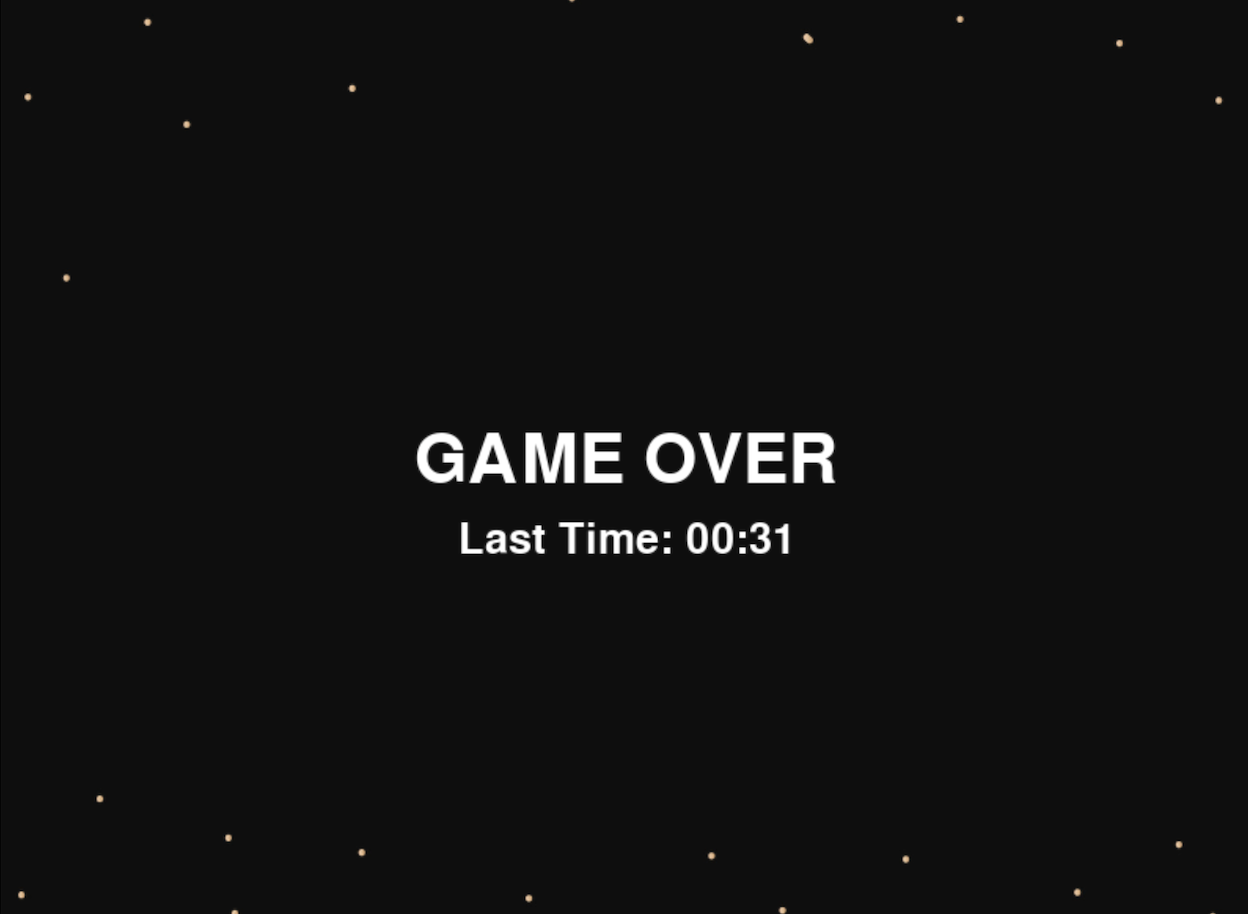
\includegraphics[scale=0.5]{figure3}
\caption{Game over screen}
\end{figure}

\end{document}
